% SOS modalities for object 49 (power drill), frame 250 -- generated from the released shards.
\begin{tikzpicture}[x=1cm,y=1cm,lab/.style={inner sep=0pt,font=\fontsize{7.5}{9}\selectfont},sub/.style={inner sep=0pt,font=\fontsize{7.5}{9}\selectfont,text=rpxSlate}]
\def\ih{2.66}
\node[anchor=north west,inner sep=0pt] at (0.00,0) {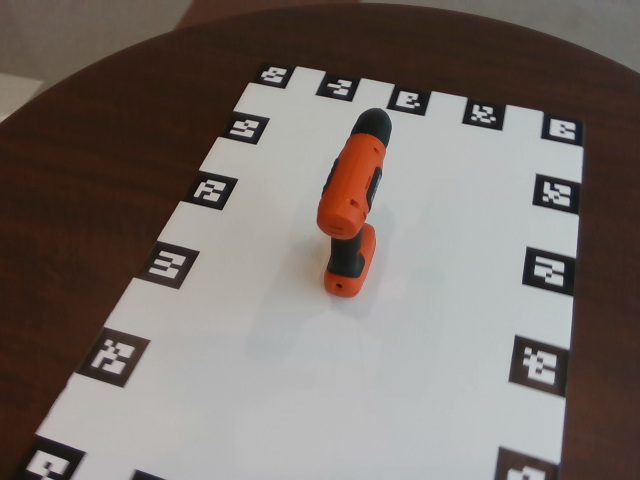
\includegraphics[width=3.55cm,height=\ih cm]{assets/images/appendix/objects/sosmod_rgb.jpg}};
\draw[rpxAccent,line width=.35pt] (0.00,0) rectangle ++(3.55,-\ih);
\node[lab,anchor=north west] at (0.00,-2.78) {\textbf{RGB}}; \node[sub,anchor=north west] at (0.00,-3.14) {D435, $640\times480$};
\node[anchor=north west,inner sep=0pt] at (3.67,0) {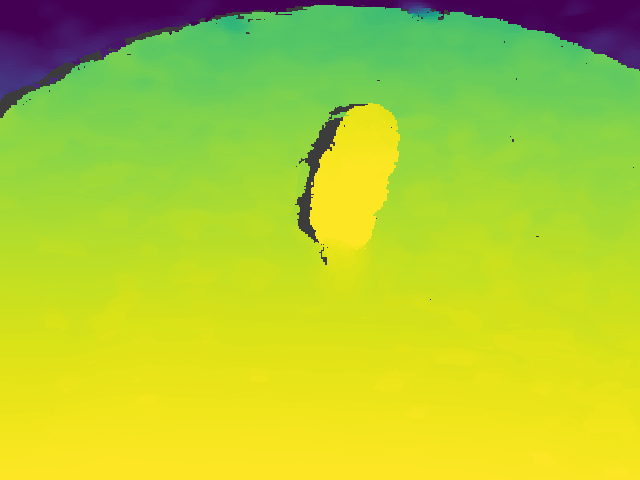
\includegraphics[width=3.55cm,height=\ih cm]{assets/images/appendix/objects/sosmod_depth.png}};
\draw[rpxAccent,line width=.35pt] (3.67,0) rectangle ++(3.55,-\ih);
\node[lab,anchor=north west] at (3.67,-2.78) {\textbf{Metric depth}}; \node[sub,anchor=north west] at (3.67,-3.14) {D435, 0.6--2.3\,m};
\shade[left color={rgb,255:red,253;green,231;blue,37},right color={rgb,255:red,68;green,1;blue,84}] (6.02,-2.83) rectangle ++(1.2,-.16); \node[sub,anchor=east] at (5.97,-2.91) {near}; \node[sub,anchor=north east] at (7.22,-3.14) {far};
\node[anchor=north west,inner sep=0pt] at (7.34,0) {
\includegraphics[width=3.55cm,height=\ih cm]{assets/images/appendix/objects/sosmod_mask.png}};
\draw[rpxAccent,line width=.35pt] (7.34,0) rectangle ++(3.55,-\ih);
\node[lab,anchor=north west] at (7.34,-2.78) {\textbf{Instance mask}}; \node[sub,anchor=north west] at (7.34,-3.14) {released label};
\node[anchor=north west,inner sep=0pt] at (11.01,0) {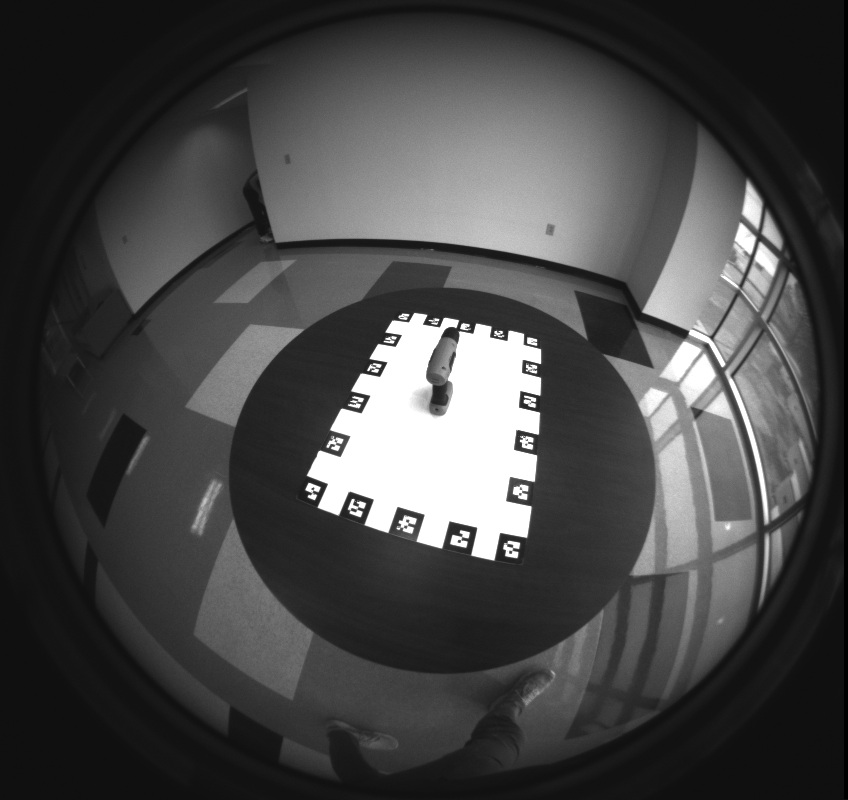
\includegraphics[width=2.82cm,height=\ih cm]{assets/images/appendix/objects/sosmod_fishl.jpg}};
\draw[rpxAccent,line width=.35pt] (11.01,0) rectangle ++(2.82,-\ih);
\node[lab,anchor=north west] at (11.01,-2.78) {\textbf{Fisheye stereo, left}}; \node[sub,anchor=north west] at (11.01,-3.14) {T265, $848\times800$};
\node[anchor=north west,inner sep=0pt] at (13.95,0) {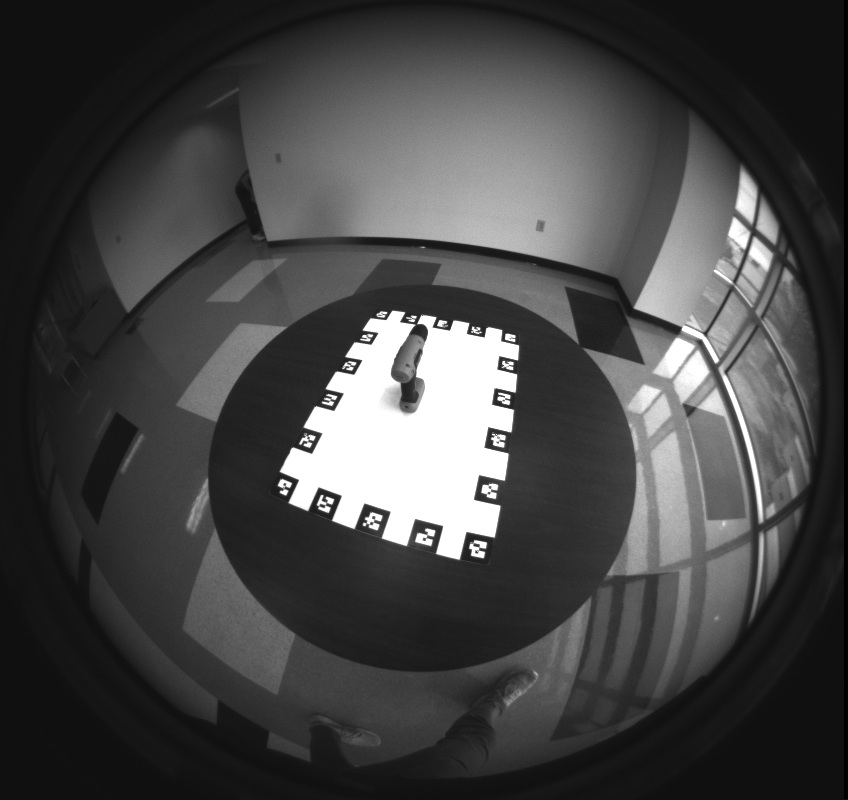
\includegraphics[width=2.82cm,height=\ih cm]{assets/images/appendix/objects/sosmod_fishr.jpg}};
\draw[rpxAccent,line width=.35pt] (13.95,0) rectangle ++(2.82,-\ih);
\node[lab,anchor=north west] at (13.95,-2.78) {\textbf{Fisheye stereo, right}}; \node[sub,anchor=north west] at (13.95,-3.14) {T265, $848\times800$};
\begin{scope}[shift={(0,-3.75)}]
\draw[rpxHair,line width=.3pt,fill=rpxPale] (0,0) rectangle (5.6,-4.0);
\begin{scope}[shift={(0,-4.0)}]
\draw[rpxAccent,line width=.45pt] plot coordinates {(1.661,0.500) (1.579,0.569) (1.494,0.634) (1.404,0.707) (1.321,0.771) (1.237,0.847) (1.152,0.931) (1.071,1.017) (0.999,1.110) (0.939,1.214) (0.892,1.324) (0.842,1.500) (0.812,1.626) (0.788,1.760) (0.780,1.883) (0.781,2.076) (0.775,2.208) (0.787,2.325) (0.808,2.452) (0.850,2.592) (0.906,2.699) (0.970,2.795) (1.045,2.893) (1.117,2.973) (1.195,3.054) (1.282,3.141) (1.369,3.220) (1.473,3.302) (1.585,3.370) (1.732,3.440) (1.929,3.525) (2.081,3.584) (2.227,3.628) (2.372,3.658) (2.525,3.682) (2.659,3.685) (2.785,3.683) (2.920,3.673) (3.047,3.661) (3.182,3.637) (3.307,3.608) (3.424,3.583) (3.544,3.539) (3.648,3.492) (3.808,3.401) (3.905,3.337) (3.994,3.261) (4.080,3.186) (4.164,3.103) (4.233,2.997) (4.287,2.887) (4.332,2.776) (4.370,2.660) (4.402,2.555) (4.434,2.451) (4.453,2.331) (4.478,2.151) (4.479,2.038) (4.469,1.923) (4.447,1.821) (4.424,1.720) (4.393,1.612) (4.344,1.523) (4.280,1.438) (4.203,1.344) (4.127,1.263) (4.052,1.187) (3.969,1.105) (3.884,1.029) (3.781,0.951) (3.675,0.886) (3.565,0.839) (3.447,0.796) (3.342,0.766) (3.238,0.733) (3.125,0.717) (3.019,0.721) (2.906,0.734) (2.789,0.757) (2.688,0.775) (2.589,0.802) (2.489,0.829) (2.400,0.866) (2.314,0.908) (2.229,0.972) (2.160,1.040) (2.086,1.111) (2.034,1.179) (1.971,1.290) (1.948,1.372) (1.930,1.463) (1.914,1.544) (1.899,1.626) (1.887,1.712) (1.878,1.796) (1.877,1.885) (1.885,1.988) (1.902,2.078) (1.910,2.166) (1.939,2.257) (1.970,2.338) (2.023,2.426) (2.081,2.500) (2.148,2.564) (2.223,2.624) (2.287,2.670) (2.348,2.711) (2.413,2.750) (2.475,2.788) (2.535,2.816) (2.603,2.842) (2.663,2.852) (2.726,2.860) (2.794,2.862) (2.852,2.859) (2.911,2.845) (2.969,2.817) (3.037,2.787) (3.094,2.744) (3.150,2.705) (3.204,2.664) (3.266,2.622) (3.323,2.575) (3.380,2.525) (3.435,2.463) (3.480,2.404) (3.515,2.345) (3.545,2.275) (3.556,2.241) (3.571,2.178) (3.575,2.110) (3.565,2.032) (3.553,1.963) (3.536,1.895) (3.527,1.823) (3.517,1.759) (3.505,1.701) (3.488,1.641) (3.474,1.594) (3.453,1.545) (3.422,1.488) (3.387,1.444) (3.345,1.407) (3.293,1.373) (3.250,1.350) (3.209,1.328) (3.172,1.319) (3.125,1.315) (3.067,1.316) (3.043,1.317) (2.991,1.318) (2.946,1.315) (2.898,1.310) (2.842,1.305) (2.786,1.297) (2.729,1.294) (2.662,1.302) (2.595,1.314) (2.558,1.322) (2.496,1.341) (2.406,1.382) (2.352,1.416) (2.313,1.454) (2.279,1.497) (2.250,1.550) (2.225,1.596) (2.205,1.647) (2.184,1.700) (2.165,1.756) (2.141,1.810) (2.120,1.870) (2.106,1.926) (2.097,1.986) (2.096,2.019) (2.097,2.084) (2.098,2.142) (2.102,2.198) (2.116,2.253) (2.137,2.295) (2.166,2.338) (2.207,2.384) (2.232,2.404) (2.279,2.445) (2.326,2.486) (2.374,2.526) (2.426,2.566) (2.474,2.599) (2.500,2.615) (2.546,2.640) (2.596,2.660) (2.647,2.674) (2.697,2.686) (2.751,2.696) (2.802,2.707) (2.852,2.717) (2.879,2.720) (2.926,2.718) (2.981,2.710) (3.035,2.698) (3.087,2.683) (3.141,2.661) (3.189,2.644) (3.234,2.626) (3.278,2.610) (3.312,2.591) (3.348,2.574) (3.389,2.545) (3.409,2.526) (3.449,2.488) (3.485,2.443) (3.520,2.393) (3.543,2.346) (3.556,2.299) (3.565,2.244) (3.566,2.190) (3.561,2.133) (3.555,2.067) (3.548,2.006) (3.541,1.947) (3.535,1.886) (3.526,1.834) (3.520,1.781) (3.509,1.719) (3.499,1.662) (3.483,1.597) (3.464,1.541) (3.454,1.509) (3.434,1.455) (3.412,1.405) (3.391,1.362) (3.366,1.317) (3.333,1.270) (3.299,1.227) (3.259,1.180) (3.220,1.139) (3.188,1.103) (3.164,1.078) (3.146,1.058) (3.131,1.044) (3.120,1.034) (3.114,1.025) (3.112,1.024) (3.110,1.026) (3.108,1.029) (3.105,1.033) (3.102,1.038) (3.098,1.041) (3.097,1.042) (3.093,1.043) (3.090,1.043)};
\draw[rpxInk,line width=.5pt] (2.68,2.00) -- ++(.24,0) (2.80,1.88) -- ++(0,.24);
\fill[tierH] (3.480,2.404) circle (1.6pt); \draw[tierH,line width=.7pt,-{Stealth[length=3.5pt]}] (3.480,2.404) -- ++(-0.612,-0.339);
\fill[rpxInk] (1.661,0.500) circle (1.2pt);
\draw[rpxInk,line width=.6pt] (0.25,0.3) -- ++(0.817,0) node[sub,midway,above=1.5pt] {0.5\,m};
\end{scope}
\node[lab,anchor=north west] at (0,-4.12) {\textbf{Camera pose}}; \node[sub,anchor=north west] at (0,-4.48) {T265, 500 frames, top view; \textcolor{tierH}{$\bullet$} frame 250 and heading, $+$ object};
\end{scope}
\node[anchor=north west,inner sep=0pt] at (5.95,-3.75) {\begin{minipage}[t]{10.82cm}\fontsize{7.5}{9.2}\selectfont\textbf{Questionnaire}\enspace{\color{rpxSlate}all released annotator responses}\par\vspace{3pt}\arrayrulecolor{rpxRule}\setlength{\tabcolsep}{3pt}\begin{tabular}{@{}l>{\raggedright\arraybackslash}p{9.17cm}@{}}\toprule
\textbf{Name} & drill / drilling machine \\[1.5pt]
\textbf{Category} & tool / home utensil / tools \\[1.5pt]
\textbf{Colour} & black / orange \\[1.5pt]
\textbf{Material} & metal / plastic \& steel / plastic \\[1.5pt]
\textbf{Function} & drilling / to build something / to put pieces of something together / to fix something / drilling holes \\\bottomrule\end{tabular}\par\vspace{4pt}{\color{rpxSlate}Canonical entry (Table~\ref{tab:sos-canonical}): \textbf{49 power drill}, tool $\cdot$ black $\cdot$ metal --- drilling.}\end{minipage}};
\end{tikzpicture}
